% 5) Methods - provide a description of the way in which you intend to address the research question.  This means describing the existing tools/systems that you will use, new tools or systems that you will build and the experiments that you will conduct.
\section{Methods}
The approach we have decided to take for the project is system-building.
Our task is to devise an internet payment architecture which fulfills our guidelines of scalability and maximizing usability.
One of the major difficulties in this task is addressing the shortcomings of the attempts we've outlined above.

Specifically, our plan is to explore a framework similar to that of Google Contributor, so we will primarily need to address the concerns of overhead and ad coverage.
Any overhead required by our system will limit its scalability, preventing widespread adoption from ever being an option.
Similarly, if our system is not able to extend to all forms of digital advertising, ad-blocking users who are used to entirely ad-free viewing will not be attracted to using it.
Hence, we must find a way to replace all advertisements (those from premium campaigns, ad networks, and ad exchanges), rather than only those from one source.

There are also some practical questions which are left to be answered, such as the feasibility of entering the advertising industry from a business standpoint, but we will consider those outside the scope of the project; our focus lies in design and implementation.

\subsection{Harpocrates}
We designed a system, Harpocrates (Greek god of silence, secrets, and confidentidality), which allows users to easily compensate publishers at a fair rate for their content.
Harpocrates is composed of a client-side browser extension for users and a server for accounting.
Furthermore, it fits into the current ad ecosystem with minimal implementation work required for publishers.

\subsubsection{Design Considerations}
Address the concerns of current adblock users
Provide an unobtrusive web browsing experience
Improve performance over the current ad delivery process
Limit the personal information of users collected
Fit into the current web ecosystem
Minimize implementation cost for publishers
Provide control over web browsing to users and publishers

\subsubsection{Architecture}
The solution relies on fact that ad exchanges are efficient marketplaces for determining the fair value for a given piece of real estate on the internet.
In order to take advantage of this fact, Harpocrates sits inline in the ``waterfall'' (Figure ~\ref{fig:waterfall}).

\begin{figure}[h]
\centering
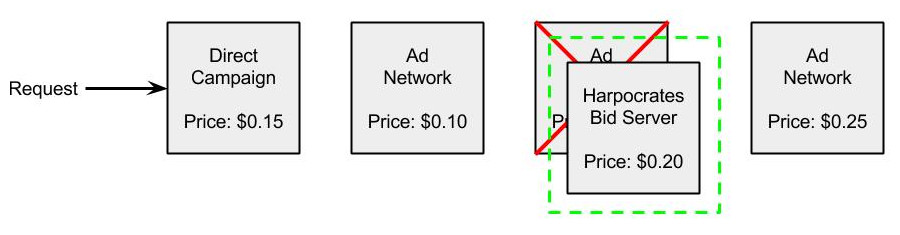
\includegraphics[width=0.5\textwidth]{waterfall}
\caption{Harpocrates sits inline with the current ad exchange ecosystem.}
\label{fig:waterfall}
\end{figure}

\begin{figure}[h]
\centering
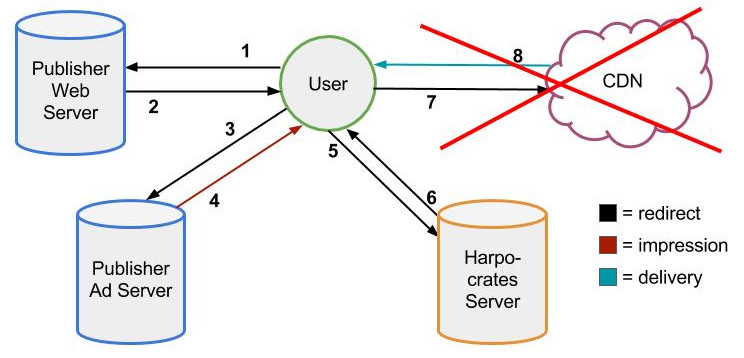
\includegraphics[width=0.5\textwidth]{harpocrates}
\caption{Harpocrates cuts out a whole roundtrip request to the ad server CDN, improving performance.}
\label{fig:waterfall}
\end{figure}

\subsubsection{User Interface}
Figure ~\ref{fig:ui}

\begin{figure}[h]
\centering
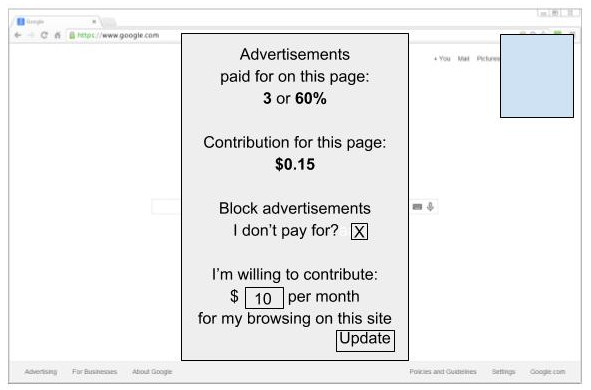
\includegraphics[width=0.5\textwidth]{ui}
\caption{For the user, Harpocrates simply requires installing a browser extension and initializing a few settings.}
\label{fig:ui}
\end{figure}

\subsection{\textit{Un}acceptable Ads}
Figure ~\ref{fig:unacceptable}

\begin{figure}[h]
\hfill
\subfigure{
\includegraphics[width=0.2\textwidth]{unacceptable_no_tolerance}}
\hfill
\subfigure{
\includegraphics[width=0.2\textwidth]{unacceptable_high_tolerance}}
\caption{\textit{Un}acceptable Ads allows the user to select their tolerance for advertisements, from 0\% (left) upwards.}
\label{fig:unacceptable}
\end{figure}

\subsection{Measurement Experiments}
Figure ~\ref{fig:load_times}

\begin{figure}[h]
\centering
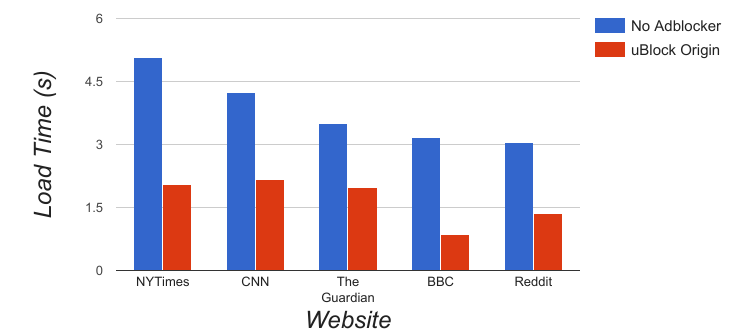
\includegraphics[width=0.5\textwidth]{load_times}
\caption{Loading times for five popular websites with and without the popular ad-blocker uBlock Origin.}
\label{fig:load_times}
\end{figure}

Figure ~\ref{fig:load_times_over_range}

\begin{figure}[h]
\centering
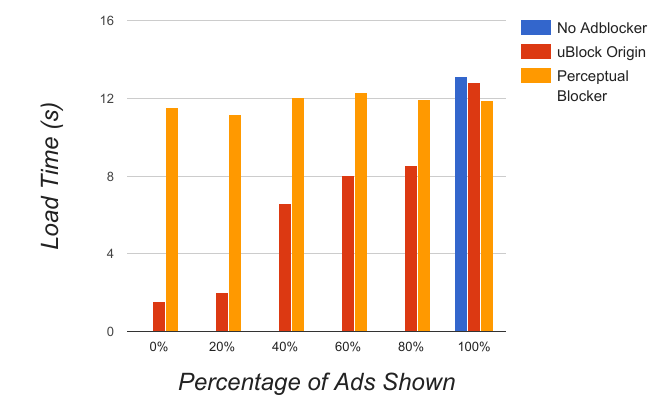
\includegraphics[width=0.5\textwidth]{load_times_over_range}
\caption{Loading times for Chicago Tribune homepage with varying levels of tolerance for ads using the \textit{Un}acceptable Ads extension (``Perceptual Blocker'') and a modified version of uBlock Origin.}
\label{fig:load_times_over_range}
\end{figure}